\documentclass[../dissertation.tex]{subfiles}

\begin{document}

\subsection{Experiment 6 - Impact of Wi-Fi Connection when using Representative Data}
\label{experiment-6}

\paragraph{Introduction} In Section \ref{exp-4} it was concluded that using a Wi-Fi connection between ROS hosts resulted in less predictable message latencies, as well as higher message latencies at all message frequencies due to the slower communication channel.

\paragraph{Objective} The aim of this experiment was to verify the results of Experiment 4 were valid when using more common message types. The two message types to be used are sensor data, and video data, as discussed previously in Section \ref{exp-5}.

\paragraph{Hypothesis} Expectations from this experiment were that the results of Experiment 4 would be exacerbated, meaning that overall latencies would be even higher than seen in Section \ref{exp-4} and the frequency at which performance starts to become worse would be lower. The higher latencies of Wi-Fi seen in Section \ref{exp-4} would be even higher by using larger message sizes, and performance would degrade even faster than in Experiment 4.

\paragraph{Materials and Methodology} This experiment was a repeat of Experiment 4 (described in Section \ref{exp-4}), except using data representative of what might be used in a typical ROS system. The data used was the same MIT Stata Center dataset used previously in Experiment 5, described in detail in Sections \ref{communication-real-data} and \ref{exp-5} - however only sensor data was evaluated as video data was too large to work with on the Raspberry Pi platform since message latencies were frequently several seconds even at very low frequencies. The implementation of this experiment required changing the message data types from what was used in Experiment 4, to what was used in Experiment 5 - thus the code was the same as used in Experiment 5\cite{Experiment5ROSbagCode}.

\paragraph{Results and Discussion} Results showed what has been classified as `good' performance at only 200Hz (see Figure \ref{exp6-sensor-wifi-all-freq-stream}). Raising the message frequency to 400Hz (and higher) introduced a significant drop in performance - from an average message latency of 23.1ms at 200Hz to 726.4ms at 400Hz, and peaking with a latency of 1721.4ms at 2000Hz (see Figure \ref{exp6-sensor-wifi-all-freq-mean}).

This leads to the conclusion that \textit{Wi-Fi is a suitable choice of communication medium, as long as suitable low message frequency is chosen so as to ensure consistent performance for the message size being used.} There was notable difference in performance at 200Hz from Ethernet (23.1ms for Wi-Fi, compared to 4.3ms for Ethernet), however as the difference was consistent throughout the message stream (see Figure \ref{exp6-sensor-wifi-all-freq-stream}) this difference can be taken in to account for future experiments.

\begin{figure}[H]
\centering
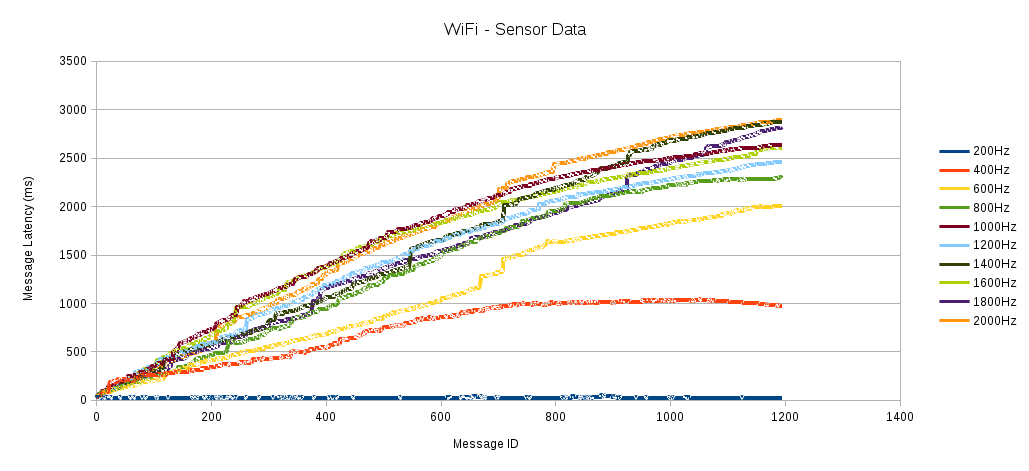
\includegraphics[width=\textwidth]{images/experiment6/sensor_data_wifi_all_freqs_stream.png}
\caption{Experiment 6 - Sensor Data Wi-Fi, All Frequencies}
\label{exp6-sensor-wifi-all-freq-stream}
\end{figure}

\begin{figure}[H]
\centering
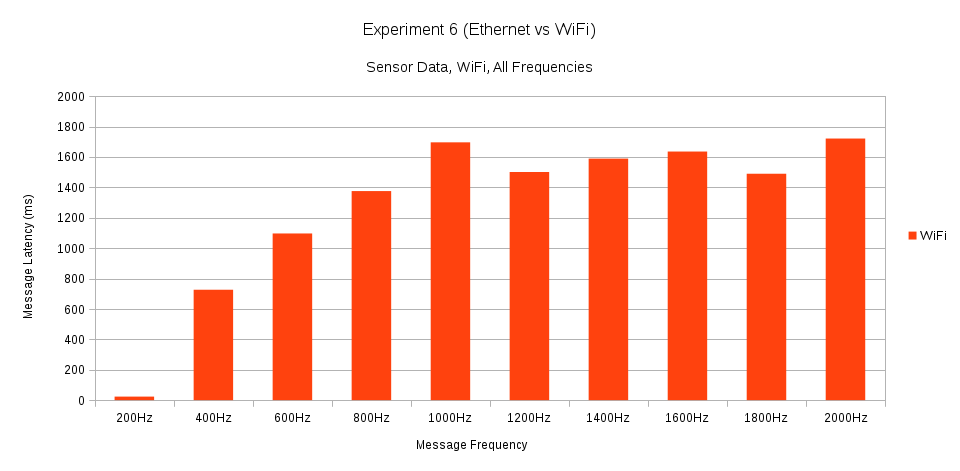
\includegraphics[width=\textwidth]{images/experiment6/sensor_data_wifi_all_freqs_mean.png}
\caption{Experiment 6 - Sensor Data Wi-Fi, All Frequencies}
\label{exp6-sensor-wifi-all-freq-mean}
\end{figure}

\paragraph{Further Investigation} After the results shown in Figure \ref{exp6-sensor-wifi-all-freq-mean} demonstrated a significant difference between message frequencies of 200Hz and 400Hz, it was decided that further runs should be conducted between these frequencies to investigate the point at which performance degrades. The extra runs conducted started at 100Hz (to gain information about performance below 200Hz), and increased in 50Hz increments up to 600Hz. The main areas of interest were 250Hz, 300Hz, and 350Hz.

As Figure \ref{exp6-sensor-wifi-more-freq-stream} shows, message stream performance was similar as seen in Figure \ref{exp6-sensor-wifi-all-freq-stream}. Certain streams exhibited consistent low latency throughout their streams, but above a certain frequency (350Hz and up in this case) performance begins to degrade. Figure \ref{exp6-sensor-wifi-more-freq-means} more clearly shows the jump in average message latency between 300Hz and 350Hz. This leads to the conclusion that \textit{for the sensor data message size (around 108kB), a suitable maximum frequency for publishing to ROS topics would be 300Hz for this message size and hardware platform.}

\begin{figure}[H]
\centering
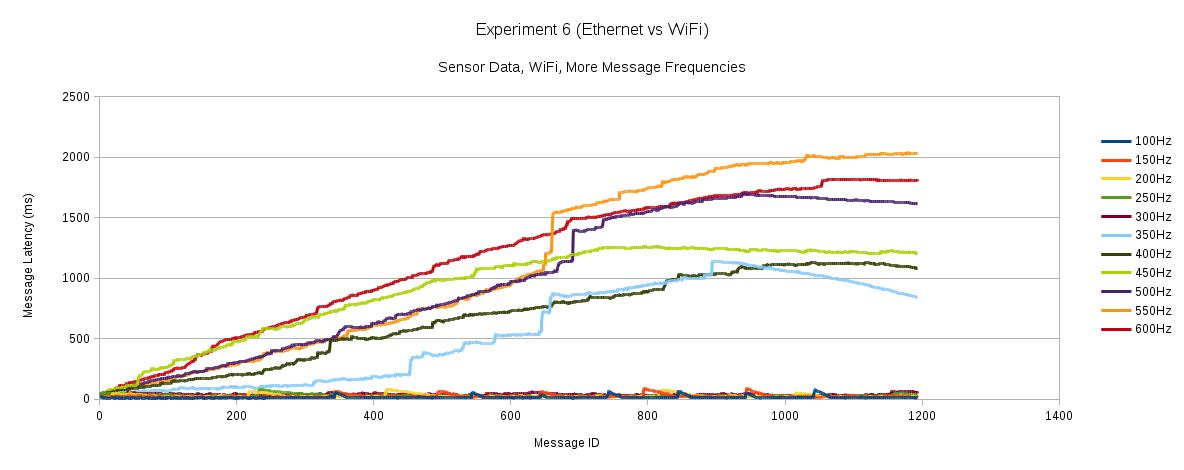
\includegraphics[width=\textwidth]{images/experiment6/sensor_data_wifi_more_freqs_stream.png}
\caption{Experiment 6 - Sensor Data Wi-Fi, More Frequencies}
\label{exp6-sensor-wifi-more-freq-stream}
\end{figure}

\begin{figure}[H]
\centering
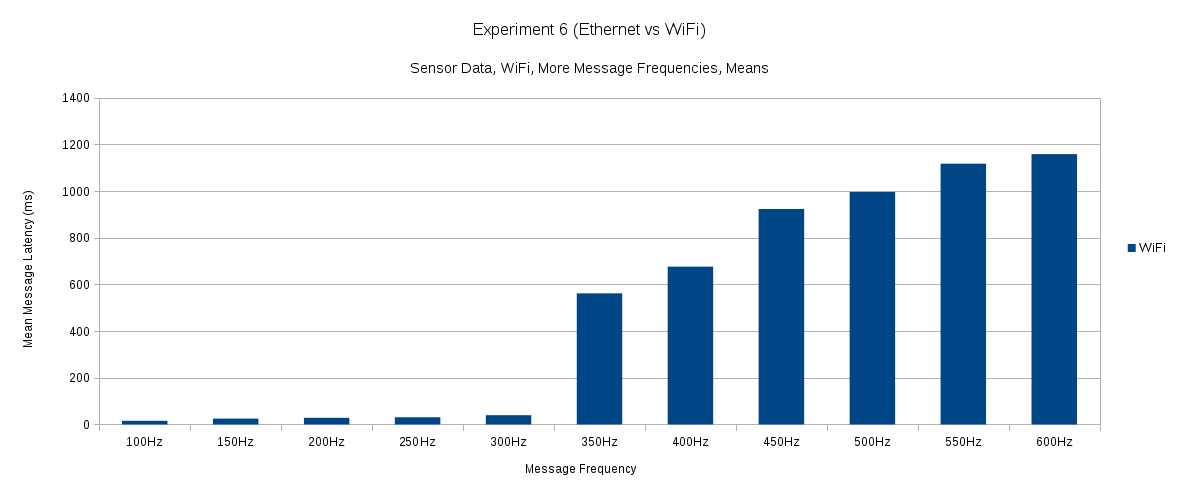
\includegraphics[width=\textwidth]{images/experiment6/sensor_data_wifi_more_freqs_means.png}
\caption{Experiment 6 - Sensor Data Wi-Fi, More Frequencies}
\label{exp6-sensor-wifi-more-freq-means}
\end{figure}


\end{document}
